\chapter{Meccanismi Differenzialmente Privati}

\section{Definizione}
La definizione seguente costituisce un formalismo più ristretto rispetto alla definizione completa, quest'ultima include un secondo parametro $\mathcal{\delta}$, la cui funzione e utilità verranno discusse in seguito.

Una trasformazione $\mathcal{M}$ è considerata $\varepsilon$-differenzialmente privata se, per ogni dataset $D_1$ e $D_2$ che differiscono al massimo per un individuo ($\norm{D_1 - D_2}_1 \le 1$) e ogni $S \subseteq \operatorname{Range}(\mathcal{M})$, vale la seguente disequazione \cite{10.1007/11681878_14}:
\begin{equation}
  \Pr[\mathcal{M}(D_1) = S] \le e^{\varepsilon} \cdot \Pr[\mathcal{M}(D_2) = S]
  \label{eq:e_differential_privacy}
\end{equation}

I termini $\Pr[\mathcal{M}(D_1) = S]$ e $\Pr[\mathcal{M}(D_2) = S]$ indicano la probabilità che il risultato dell'applicazione del meccanismo $\mathcal{M}$ su $D_1$ e $D_2$ risulti nell'output $S \in \operatorname{Range}(\mathcal{M})$.
Il termine $e^\varepsilon, \varepsilon > 0$ rappresenta un coefficiente che indica quanto le due probabilità possono differire tra di loro, in particolare per valori di $\varepsilon$ vicini a $0$ le probabilità sono simili; all'aumentare di $\varepsilon$ la differenza tra le due probabilità può aumentare.

Considerando che i due database $D_1$ e $D_2$ differiscono per un solo individuo, essi sono intercambiabili; ciò rende la definizione simmetrica. Vale quindi anche:
\begin{equation}
  e^{-\varepsilon} \cdot \Pr[\mathcal{M}(D_2) = S] \le \Pr[\mathcal{M}(D_1) = S] \le e^{\varepsilon} \cdot \Pr[\mathcal{M}(D_2) = S]
  \label{eq:e_differential_privacy_symm}
\end{equation}

\subsubsection{Un esempio pratico}
\label{ex:coint_toss}
Si supponga di volere condurre un sondaggio su una popolazione ponendo la domanda: "Nell'ultimo anno hai guidato un veicolo sotto l'influenza di alcol o stupefacenti?".
Ovviamente, una persona alla quale viene posta direttamente questa domanda tenderà a mentire allo scopo di proteggere la propria privacy e evitare di autoincriminarsi. In questa istanza può rendersi utile l'applicazione di un meccanismo differenzialmente privato.

Per ovviare a questa limitazione del processo di raccolta dati, si richiede ai partecipanti di lanciare una moneta senza mostrare il risultato:
\begin{itemize}
    \item se il risultato è testa il soggetto risponde alla domanda in modo sincero
    \item se il risultato è croce il soggetto lancia una seconda moneta: su testa risponde "Si", su croce "No"
\end{itemize}

\begin{tikzpicture}
\node (start) [draw,font=\scriptsize,rectangle,align=center,text width=0.2*\textwidth] {Nell'ultimo anno hai guidato un veicolo sotto l'influenza di alcol o stupefacenti?};

\node (dec1) [draw,font=\scriptsize,rectangle,right=2.5cm of start.center] {Lancia moneta};
\node (heads1) [draw,minimum height=1cm,minimum width=1cm,font=\scriptsize,circle,above=1cm of dec1.center] {Testa};
\node (tails1) [draw,minimum height=1cm,minimum width=1cm,font=\scriptsize,circle,below=1cm of dec1.center] {Croce};

\node (heads2) [draw,minimum height=1cm,minimum width=1cm,font=\scriptsize,circle,right=2cm of dec1.center] {Testa};
\node (truth) [draw,font=\scriptsize,rectangle,above=of heads2.north,right=2cm of heads1.center] {Verità};
\node (dec2) [draw,font=\scriptsize,rectangle,below=of heads2.south,right=2cm of tails1.east,anchor=center] {Lancia moneta};

\node (tails2) [draw,minimum height=1cm,minimum width=1cm,font=\scriptsize,circle,right=1cm of dec2.east] {Croce};
\node (out1) [draw,font=\scriptsize,rectangle,above=of tails2.north,right=of heads2.east] {Rispondi "Si"};
\node (out2) [draw,font=\scriptsize,rectangle,right=1cm of tails2.east] {Rispondi "No"};

\draw [-latex] (start.east) -- (dec1.west);
\draw [-latex] (dec1.north) -- (heads1.south);
\draw [-latex] (dec1.south) -- (tails1.north);
\draw [-latex] (tails1.east) -- (dec2.west);
\draw [-latex] (heads1.east) -- (truth.west);
\draw [-latex] (dec2.north) -- (heads2.south);
\draw [-latex] (dec2.east) -- (tails2.west);
\draw [-latex] (tails2.east) -- (out2.west);
\draw [-latex] (heads2.east) -- (out1.west);
\end{tikzpicture}

Questo processo introduce un elemento casuale alla risposta di un singolo soggetto, offrendo all'individuo una negazione plausibile contro eventuali accuse e impedendo a terze parti di discriminare sulla base delle risposte \cite{Warner01031965}.

Nel complesso, riscrivendo i risultati nei termini della definizione si ottiene:
\begin{itemize}
    \item $\Pr[\mathcal{M}(Si) = Si] = 0.75$, $\Pr[\mathcal{M}(Si) = No] = 0.25$
    \item $\Pr[\mathcal{M}(No) = Si] = 0.25$, $\Pr[\mathcal{M}(No) = No] = 0.75$
\end{itemize}

Considerati questi risultati si può affermare che il meccanismo illustrato è $\ln{3}$-differenzialmente privato; si può dimostrare partendo dalla definizione \eqref{eq:e_differential_privacy} che:
\begin{align*}
    \frac{\Pr[\mathcal{M}(D_1) = S]}{\Pr[\mathcal{M}(D_2) = S]
    } &\le e^{\varepsilon}\\
    \frac{\Pr[\mathcal{M}(Si) = Si]}{\Pr[\mathcal{M}(Si) = No]} &\le 3 = \frac{\Pr[\mathcal{M}(No) = No]}{\Pr[\mathcal{M}(No) = Si]}
\end{align*}

Il meccanismo illustrato dimostra in termini semplici come la privacy differenziale possa agire sui dati per proteggere la privacy dei partecipanti che aderiscono a essere inseriti in una raccolta di dati. Come specificato in precedenza, questo processo garantisce negazione plausibile sul contenuto della risposta ai soggetti partecipanti; non fornisce tuttavia la possibilità di negare di aver partecipato al sondaggio. Al contrario, la privacy differenziale è applicabile solamente a distribuzioni di dati basate su sistemi di interrogazione che generano risultati aggregati.

\subsection{Quantificazione della conoscenza dell'attaccante}
Il parametro $\varepsilon$ presente nella definizione di $\varepsilon$-DP può essere interpretato come una misura del livello massimo di conoscenza che un potenziale attaccante può guadagnare osservando i risultati di un'interrogazione del meccanismo differenzialmente privato.

Prendendo come riferimento un attaccante che conosce l'intero database eccetto il soggetto target si può modellare il suo punto di vista considerando due possibili dataset: $D_{in}$ contiene il target mentre $D_{out}$ no; l'obiettivo dell'attaccante è capire quale dei due database è quello reale.

Nel modello dell'attaccante si può esprimere il sospetto che il database $D$ sia $D_{in}$ come $\Pr[D = D_{in}] = 1 - \Pr[D = D_{out}]$. Si supponga ora che l'attaccante abbia osservato che il meccanismo DP applicato a $D$ restituisce l'output $O$: si può esprimere la probabilità che $D = D_{in}$ dopo aver osservato l'output come $\Pr[D = D_{in} | \mathcal{M}(D) = O]$; applicando il teorema di Bayes si ottiene un'espressione che permette di quantificare il livello di sospetto $Pr[D = Din|M(D) = O]$ che l'attaccante ha dopo aver osservato l'output $O$.
\begin{equation}
\label{eq:bayes_susp}
    \Pr[D = D_{in} | \mathcal{M}(D) = O] = \frac{\Pr[D = D_{in}] \cdot \Pr[\mathcal{M}(D) = O | D = D_{in}]}{\Pr[\mathcal{M}(D) = O]}
\end{equation}
Il termine $\Pr[D = D_{in}]$ è il sospetto iniziale e il termine $\Pr[\mathcal{M}(D) = O | D = D_{in}]$ può essere riscritto come $\Pr[\mathcal{M}(D_{in}) = O]$ indicando la probabilità che il meccanismo $\mathcal{M}$ applicato a $D_{in}$ restituisca $O$. Mentre i primi due termini sono conosciuti, il termine $\Pr[\mathcal{M}(D) = O]$ è sconosciuto; per rimediare si può considerare il rapporto tra i due sospetti aggiornati all'output $O$.
\begin{equation}
\label{eq:bayes_susp_ratio}
    \frac{\Pr[D = D_{in} | \mathcal{M}(D) = O]}{\Pr[D = D_{out} | \mathcal{M}(D) = O]} = \frac{\Pr[D = D_{in}]}{\Pr[D = D_{out}]} \cdot \frac{\Pr[\mathcal{M}(D_{in}) = O]}{\Pr[\mathcal{M}(D_{out}) = O]}
\end{equation}
In questa espressione emerge il termine $\frac{\Pr[\mathcal{M}(D_{in}) = O]}{\Pr[\mathcal{M}(D_{out}) = O]}$, la definizione di $\varepsilon$-DP \eqref{eq:e_differential_privacy} limita il rapporto come segue:
\begin{equation}
\label{eq:e_dp_bounds}
    e^{-\varepsilon} \le \frac{\Pr[\mathcal{M}(D_{in}) = O]}{\Pr[\mathcal{M}(D_{out}) = O]} \le e^{\varepsilon}
\end{equation}
Applicando all'equazione \eqref{eq:bayes_susp_ratio} si ottiene:
\begin{equation}
\label{eq:mid_information_gain}
    e^{-\varepsilon} \cdot \frac{\Pr[D = D_{in}]}{\Pr[D = D_{out}]} \le \frac{\Pr[D = D_{in} | \mathcal{M}(D) = O]}{\Pr[D = D_{out} | \mathcal{M}(D) = O]} \le e^{\varepsilon} \cdot \frac{\Pr[D = D_{in}]}{\Pr[D = D_{out}]} 
\end{equation}
Applicando le sostituzioni $\Pr[D = D_{out}] = 1 - \Pr[D = D_{in}]$ e $\Pr[D = D_{out} | \mathcal{M}(D) = O] = 1 - \Pr[D = D_{in} | \mathcal{M}(D) = O]$ e riorganizzando i termini si ottiene:
\begin{equation}
\label{eq:information_gain}
    \frac{\Pr[D = D_{in}]}{e^\varepsilon + (1 - e^\varepsilon) \cdot \Pr[D = D_{in}]} \le \Pr[D = D_{in} | \mathcal{M}(D) = O] \le \frac{e^\varepsilon \cdot \Pr[D = D_{in}]}{1 + (e^\varepsilon - 1) \cdot \Pr[D = D_{in}]}
\end{equation}
Per i passaggi della trasformazione, consultare l'appendice \ref{eqd:information_gain_derivation}.

Tracciando il grafico dell'espressione risultante al variare di $\varepsilon$ si può notare come il guadagno di informazione potenziale possa aumentare drasticamente per valori di $\varepsilon$ alti.
\begin{figure}[H]
    \centering
    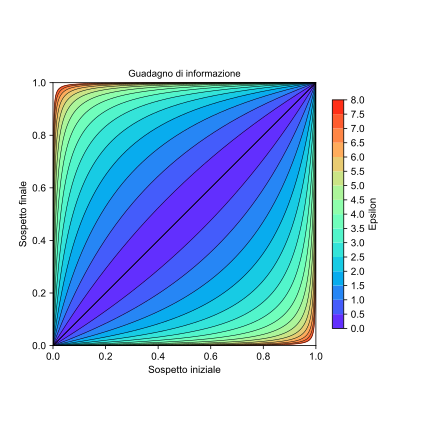
\includegraphics[scale=0.8]{plots/information_gain.pdf}
    \caption{Guadagno di informazione sul dataset al variare di epsilon}
\end{figure}

\section{Meccanismo di Laplace}
Le query più comuni che vengono effettuate su database sono di tipo numerico, precisamente sono funzioni del tipo $f \colon \mathbb{N}^{|\mathcal{X}|} \to \mathbb{R}^k$, dove $\mathcal{X}$ rappresenta l'universo di possibili record in un database $x$.

Per rendere questa tipologia di query differenzialmente privata con il meccanismo di Laplace si aggiunge rumore campionato da una distribuzione di Laplace:
\begin{align}
\label{eq:laplace_distribution}
    Lap(x|\mu,b) = \frac{1}{2b}\exp\left({-\frac{|x-\mu|}{b}}\right)
\end{align}

\begin{figure}[H]
    \centering
    \includegraphics[scale=0.5]{plots/laplace_pdf.pdf}
    \caption{Distribuzione di Laplace}
\end{figure}

\subsection{Definizione}
Si consideri una qualsiasi funzione $f \colon \mathbb{N}^{|\mathcal{X}|} \to \mathbb{R}^k$, il meccanismo di Laplace è definito:
\begin{equation}
\label{eq:laplace_mechanism}
    \mathcal{M}_L(x, f(\cdot), \varepsilon) = f(x) + (Y_1, \dots, Y_k)
\end{equation}
dove i parametri $Y_i$ sono valori campionati da una distribuzione di Laplace. Per illustrare la calibrazione della distribuzione utilizzata è necessario introdurre alcuni concetti.

\subsubsection{Distanza tra database}
Si considerino due database $x, y \in \mathbb{R}^{|\mathcal{X}|}$.
Per definire la distanza tra i due database si fa uso della norma $\ell_1$, dove la norma $\ell_1$ di un database è definita come:
\begin{equation}
\label{eq:l1_norm}
    ||x||_1 = \sum_{i=1}^{|\mathcal{X}|} |x_i|
\end{equation}
La distanza $\ell_1$ tra due database $x$ e $y$ è $||x - y||_1$.

In questo caso $||x||_1$ è una misura del numero di record contenuti nel database e $||x - y||_1$ rappresenta quanti record sono diversi tra $x$ e $y$.

\subsubsection{Sensitività di una funzione}
La sensitività di una funzione è un valore che indica la magnitudine massima che un cambiamento dei dati di un singolo individuo può causare sul risultato della funzione considerata; questo valore verrà utilizzato come parametro per calibrare la quantità di rumore che il meccanismo aggiungerà ai risultati delle query.

La sensitività $\ell_1$ è definita come:
\begin{equation}
    \Delta f = \max_{\substack{x,y \in \mathbb{N}^{|\mathcal{X}|}\\||x - y||_1 = 1}} ||f(x) - f(y)||_1
\end{equation}

Utilizzando la sensitività della funzione in considerazione si calibra la scala (parametro $b$) della distribuzione di Laplace come $Lap(x|0,\Delta f/\varepsilon)$. Per la dimostrazione che l'utilizzo di questa distribuzione crea un meccanismo che rispetta $\varepsilon$-privacy differenziale consultare \ref{proof:laplace_mechanism}

\subsection{Limitazione del contributo}
Si supponga di avere a disposizione un dataset che raccoglie le lamentele poste dai clienti di un'azienda tramite un modulo di feedback e di voler creare un report sul numero di lamentele poste al giorno; si decide di applicare il meccanismo di Laplace per anonimizzare i risultati dell'analisi.

Il primo passo per creare un meccanismo di Laplace differenzialmente privato è calcolare la sensitività della funzione in considerazione. Dato che si tratta di un'operazione di conteggio, intuitivamente si può pensare che questo valore sia pari a 1; tuttavia è necessario considerare la \textit{contribuzione massima} che un singolo utente può apportare al conteggio per valutare correttamente casi in cui un individuo presenta più di una lamentela al giorno.

Se si considerasse $\Delta f = 1$ e quindi un parametro di scala per la distribuzione di Laplace pari a $b = \frac{1}{\varepsilon}$ si otterrebbe un meccanismo $x\varepsilon$-differenzialmente privato, dove $x$ corrisponde alla massima contribuzione che un singolo individuo può apportare al dataset. Supponendo un dataset di 500 unità con un utente che ha posto 5 lamentele, utilizzando $\Delta f = 1$ si otterrebbero due distribuzioni di probabilità con rapporto massimo di $e^{5\varepsilon}$, violando quindi la definizione di privacy differenziale.

Si riporta di seguito il grafico che mostra le due distribuzioni di probabilità e il loro rapporto.
\begin{figure}[H]
    \centering
    \includegraphics[scale=0.7]{plots/double_laplace_pdf.pdf}
    \caption{Distribuzioni di Laplace per dataset con e senza utente con multiple lamentele}
\end{figure}

Per rispettare i requisiti della privacy differenziale è necessario utilizzare la sensitività della funzione di conteggio tenendo conto della possibilità di avere multipli record legati a un singolo individuo.

\subsubsection{Scelta dei limiti}
Generalizzando, il problema ricade sulle caratteristiche del particolare dominio di applicazione; si rende quindi necessario l'intervento di un esperto del dominio allo scopo di definire un ragionevole limite massimo alla sensitività; in fase di analisi sarà necessario limitare il conteggio dei record relativi a un singolo individuo.









\newpage
Step successivi:\\
analisi fatta finora prevede un modello interattivo\\
considerazione su modello distribuito e locale\\
considerazione su caching e possibilità di ripetere query\\